\documentclass[10pt]{article}

\usepackage[margin=1in]{geometry}
\usepackage{amsmath}
\usepackage{amssymb}
\usepackage{graphicx}
\usepackage{apacite}

\renewcommand{\baselinestretch}{2}

\newcommand{\clr}{\operatorname{clr}}
\newcommand{\N}{\operatorname{N}}
\newcommand{\cov}{\operatorname{cov}}
\newcommand{\var}{\operatorname{var}}

\DeclareMathOperator*{\argmin}{arg\,min}
\DeclareMathOperator{\tr}{tr}

\title{Limitations of Graph Selection from High-Dimensional Compositional Data}
\author{Camden Lopez \\
\small{Department of Statistics, Oregon State University, Corvallis, OR 97331, USA} \\
\small{\textit{email:} camden.lopez@oregonstate.edu}}
\date{May 2017}

\begin{document}
\pagenumbering{gobble}
\maketitle

\begin{abstract}
Microbial abundance data produced by high-throughput genomic sequencing techniques such as 16S amplicon sequencing can be used to investigate ecological relationships among microbes. The data require special methods for analysis because they are both compositional and high-dimensional. One recently proposed method infers conditional dependence relationships within a microbial community based on log-ratio transformed abundances and graph selection via graphical lasso or neighborhood selection. The method relies on the covariance matrix for the log-ratio transformed data being approximately equal to the covariance matrix for the log-absolute abundances. Two limitations of using compositional data in this setting are that any given covariance structure for the log-ratio transformed abundances could correspond to a wide range of log-absolute abundance covariances representing diverse conditional dependence relationships, and some log-absolute abundance covariance structures can result in misleading graph inferences based on the log-ratio data.
\end{abstract}

\clearpage
\setcounter{page}{1}
\pagenumbering{arabic}

\subsection*{Introduction}

This work was motivated by the problem of inferring microbial interaction networks from compositional data. High-throughput sequencing methods such as 16S amplicon sequencing produce count data representing the abundances of microbial operational taxonomic units (OTUs) in a collection of samples. The counts are assumed to be proportional to the absolute abundances of the OTUs, but the sample preparation and sequencing process introduce biases such that the total sample counts do not accurately reflect the total abundance of microbes in the samples. Therefore, only relative abundances within a sample are meaningful, and the data are considered compositional \cite{gloor,tsilimigras}. The data for each sample essentially amount to a vector of proportions which sum to one.

John Aitchison \citeyear{aitchison} is widely cited for the theory and methodology he developed for compositional data analysis. Microbial abundance data present a new challenge in that they are high-dimensional, with the number of OTUs often greater than the number of samples, and sparse, with many zero counts.

Given a set of microbial abundance data, one goal for analysis is sometimes to determine which OTUs appear to interact or have some kind of association. Associations among variables are often quantified using correlation, but correlation analysis of proportions making up a composition can produce spurious results because of the sum-to-one constraint. Several methods, such as SparCC \cite{friedmanjon}, have been developed to perform correlation analysis in a manner which accounts for the compositionality.

A different approach is taken with SPIEC-EASI \cite{kurtz}, which aims to infer a graph representing conditional dependence relationships among OTU absolute abundances based on relative abundance data. The proposed method involves a log-ratio transformation commonly used with compositional data. Based on an assumption that the covariance matrix of the transformed data is a good estimate of the covariance matrix of the log-absolute abundances, one of two graph selection techniques is applied to the transformed data. Here I focus on the graphical lasso technique.

Considering how relative abundances provide limited information about absolute abundances, one would expect there to be limitations in any method which claims to reliably recover absolute abundance relationships based on compositional data. I investigated the limitations of graph selection as proposed by Kurtz et al. \citeyear{kurtz} and attempted to characterize the situations where where it works well and those where it does not.

\subsection*{Graph Selection from Compositional Data}

Let $\mathrm{Y}$ be an $n \times p$ matrix of non-negative OTU count data such as that obtained from 16S amplicon sequencing, consisting of $n$ samples and $p$ OTUs. Element $y_{ij}$ is the count for OTU $j$ in sample $i$. The sample totals are uninformative, and one would typically normalize each sample by its total to obtain proportions $x_{ij} = y_{ij} / \sum_{j=1}^p y_{ij}$. Aitchison \citeyear{aitchison} suggested that compositional data be analyzed using log-ratios, and Kurtz et al. \citeyear{kurtz} use the centered log-ratio (clr) transformation, which has the advantage that it treats the components symmetrically (that is, it doesn't require arbitrarily choosing a reference component). For compositional vector $x = (x_1, \dots, x_p)$ with geometric mean $g(x) = \left(\prod_{i=1}^p x_i\right)^{1/p}$,
\begin{equation}
\label{e:clr}
\begin{split}
z = \clr(x) &= \left( \log \frac{x_1}{g(x)}, \dots, \log \frac{x_p}{g(x)} \right) \\
&= \left( \log x_1 - \frac{1}{p} \sum_{i=1}^p \log x_i, \dots, \log x_p - \frac{1}{p} \sum_{i=1}^p \log x_i \right)
\end{split}
\end{equation}

The result of the clr transformation is invariant to arbitrary scaling of the input vector, so that if $x$ is a vector of relative proportions obtained from observed abundances $y$, which are proportional to absolute abundances $w$, then $\clr(x) = \clr(y) = \clr(w)$.

Let $\mathrm{Z}$ be the matrix obtained by clr transformation of the rows of $\mathrm{Y}$. (Sequencing data typically have many zero counts which would make the clr transformation impossible, so it is necessary to add a pseudo count of 1 or by some other means make all abundances strictly positive.) A row of $\mathrm{Z}$ represents the distances of each OTU's abundance in a sample from the mean of the sample, on the log scale, and it contains all of the information that the original abundance observations contained, assuming the total observed abundance was uninformative.

A microbial interaction network can be inferred based on the graphical model representation of the log-absolute microbial abundances. Let $W = (W_1, \dots, W_p)$ be a random vector of strictly positive absolute abundances. The undirected graphical model representation of $\log W = (\log W_1, \dots, \log W_p)$ has one node for each $\log W_i$, $i = 1, \dots, p$, and an edge between node $i$ and node $j$, $i \ne j$, if and only if $\log W_i$ and $\log W_j$ are dependent (the distribution of one depends on the value of the other) conditional on the values of $\{\log W_k : k \ne i, k \ne j\}$. The lack of an edge between nodes $i$ and $j$ indicates conditional independence between $\log W_i$ and $\log W_j$.

Following the notation of Aitchison \citeyear{aitchison}, let $\Omega = \cov(\log W)$ be the population covariance matrix for the log-absolute abundances and $\Gamma = \cov(Z) = \cov(\clr W)$ be the covariance matrix for clr-transformed abundances. If $\log W \sim \N(\mu, \Omega)$, then $\log W_i$ and $\log W_j$ are conditionally dependent if and only if the $(i,j)$ entry of $\Omega^{-1}$ is non-zero, with the sign of the entry corresponding to a linear conditional relationship of the opposite sign. The graphical lasso \cite{friedmanjer} is one method for selecting non-zero entries of $\Omega^{-1}$ in the high-dimensional setting (possibly $n < p$) when $\Omega^{-1}$ is assumed to be sparse.

Graphical lasso estimates a sparse $\Omega^{-1}$ by minimizing the multivariate normal log-likelihood with a penalty on the $l_1$ norm of $\Omega^{-1}$. The graphical lasso estimate is
\begin{equation}
\label{e:glasso}
\widehat{\Omega^{-1}}_{\text{glasso}} = \argmin_{\Omega^{-1}} \left[ -\log \det(\Omega^{-1}) + \tr(\Omega^{-1} \hat{\Omega}) + \lambda \lVert \Omega^{-1} \rVert_1 \right]
\end{equation}
with $\Omega^{-1}$ restricted to positive definite matrices. $\hat{\Omega}$ is the maximum likelihood estimate of $\Omega$, $\lVert \Omega^{-1} \rVert_1 = \sum_{i,j} \lvert (\Omega^{-1})_{ij} \rvert$ is the $l_1$ norm of $\Omega^{-1}$, and $\lambda$ is the so-called lasso penalty parameter controlling the sparsity of $\widehat{\Omega^{-1}}_{\text{glasso}}$.

With only the compositional data $\mathrm{Y}$ and its clr form $\mathrm{Z}$ at hand, $\hat{\Omega}$ is unavailable. However, for many settings, $\hat{\Omega} \approx \hat{\Gamma}$, where $\hat{\Gamma}$ is the estimate of $\Gamma$ calculated from $\mathrm{Z}$ in the same way that $\hat{\Omega}$ would be calculated from the log-absolute abundances, were they available. Substituting $\hat{\Gamma}$ for $\hat{\Omega}$ into (\ref{e:glasso}) results in the sparse estimate of $\Omega^{-1}$ that will be considered here:
\begin{equation}
\widehat{\Omega^{-1}} = \argmin_{\Omega^{-1}} \left[ -\log \det(\Omega^{-1}) + \tr(\Omega^{-1} \hat{\Gamma}) + \lambda \lVert \Omega^{-1} \rVert_1 \right]
\end{equation}

Conditional dependence relationships among the log-absolute abundances are inferred based on the non-zero entries of $\widehat{\Omega^{-1}}$.

\subsection*{Covariance Properties}

From (\ref{e:clr}), $\clr(W) = \mathrm{G} \log W$ where $\mathrm{G} = \mathrm{I}_p - \frac{1}{p}\mathrm{J}$, $\mathrm{I}_p$ is the $p \times p$ identity matrix, and $\mathrm{J}_p$ is the $p \times p$ matrix of all ones. Therefore,
\begin{equation}
\Gamma = \cov(\mathrm{G} \log W, \mathrm{G} \log W) = \mathrm{G} \Omega \mathrm{G}
\end{equation}
The same relation holds for empirical covariances: $\hat{\Gamma} = \mathrm{G} \hat{\Omega} \mathrm{G}$. In the following discussion, $\Omega$ and $\Gamma$ can be understood to refer to either empirical or population covariances. The entries of $\Gamma$ are related to the entries of $\Omega$ by
\begin{equation}
\label{e:entries}
\gamma_{ij} = \omega_{ij} - \overline{\omega}_{i\cdot} - \overline{\omega}_{j\cdot} + \overline{\omega}_{\cdot\cdot}
\end{equation}
where $\overline{\omega}_{i\cdot}$ is the average of entries in the $i$th row of $\Omega$, and $\overline{\omega}_{\cdot\cdot}$ is the average of all entries of $\Omega$. Equation (\ref{e:entries}) makes it evident that all rows and columns of $\Gamma$ sum to zero. $\Omega$ has $p(p+1)/2$ free parameters. As a result of the sum-to-zero constraint, $\Gamma$ has $p$ fewer parameters, for a total of $p(p-1)/2$.

As noted above, the estimate $\widehat{\Omega^{-1}}$ relies on the approximation $\hat{\Omega} \approx \hat{\Gamma}$. Some simple examples illustrate how this approximation depends on the structure of $\Omega$. When the log abundances are all uncorrelated and the marginal variances are all equal to $\omega$, $\overline{\omega}_{i\cdot} = \overline{\omega}_{j\cdot} = \overline{\omega}_{\cdot\cdot} = \frac{1}{p}\omega$ and $\gamma_{ij} - \omega_{ij} = -\frac{1}{p}\omega$ for all $i$ and $j$. The correlation among the log abundances induced by the clr transformation is only $-\frac{1}{p}$, so for large $p$, the effect of clr transformation is negligible.

Suppose one variance is larger than the others. Let $\omega_{11} = M\omega$, with $M > 1$. When the variance in one abundance variable is so much larger than the others that it dominates the variance in the total abundance, there will be a negative correlation induced between that variable and the others when considered as a composition or following a clr transformation. For $p = 64$, the induced correlation between the variance-dominating component and the others (that is, the correlation obtained from converting $\Gamma$ to the corresponding correlation matrix) is $-0.08$ when $M = 25$, $-0.16$ when $M = 100$, and $-0.30$ when $M = 400$.

Under some assumptions about how many strong correlations there are among the log abundances, the approximation $\Omega \approx \Gamma$ improves as $p$ increases. If the sums of the rows of $\Omega$ grow slower than $p$ as $p$ increases, then each $\overline{\omega}_{i\cdot}$ and $\overline{\omega}_{\cdot\cdot}$ diminish so that $\vert \gamma_{ij} - \omega_{ij} \rvert$ also diminishes. In the microbial setting, it may be reasonable to assume that for any particular OTU, the variance of its log abundance plus the covariances between it and other OTUs grows slower than $p$ as more OTUs are included in the data.

If all $\overline{\omega}_{i\cdot}$ are approximately equal to $\overline{\omega}_{1\cdot}$, then $\gamma_{ij} - \omega_{ij} \approx -\overline{\omega}_{1\cdot}$, and if $\overline{\omega}_{1\cdot}$ is positive and non-negligible compared to the variances $\omega_{11}, \dots, \omega_{pp}$, then this can represent a substantial distortion of the covariances. In simulations described later, it was found that graph selection performs worse in this type of situation.

Another situation where the covariances become substantially distorted is when some $\overline{\omega}_{i\cdot}$ is much larger than the others. This occurs when, for example, one variance $\omega_{ii}$ is much larger than the others, so that the total abundance in each realization of $\log W$ is strongly influenced by the value of $\log W_i$. In that case, $\gamma_{ij} - \omega_{ij}$ tends to be a relatively large negative value for all $j = 1, \dots, p$. If $\log W_i$ and $\log W_j$, $i \ne j$, are uncorrelated, then the clr transformation induces a negative correlation in $\clr W_i$ and $\clr W_j$. This negative correlation would be observed in the proportions $X_i$ and $X_j$ as well (and is the type of spurious correlation which methods such as SparCC are designed to circumvent). When the abundances become compositional instead of absolute, if one component dominated the basis variance, then its abundance relative to other components will also dominate the composition and induce negative correlations.

\subsection*{Alternative Basis Covariances}

Let $\mathcal{S}_p$ be the set of symmetric $p \times p$ matrices with real entries, which is a space with $p(p+1)/2$ dimensions. Let $\mathrm{T}_p: \mathcal{S}_p \rightarrow \mathcal{S}_p$ be the transformation defined by $\mathrm{T}_p(\Omega) = \mathrm{G} \Omega \mathrm{G}$. $\mathrm{T}_p$ is a linear transformation with rank $p(p-1)/2$. For each $\Gamma$ representing the covariance matrix for clr-transformed abundances, there is not a unique $\Omega$ for which $\Gamma = \mathrm{T}_p(\Omega)$ but rather a $p$-dimensional space of such $\Omega$ matrices. We can characterize that space with the kernel of $\mathrm{T}_p$, $\ker(\mathrm{T}_p) = \{\Psi \in \mathcal{S}_p: \mathrm{G} \Psi \mathrm{G} = 0_{p \times p}\}$, which, it turns out, consists of matrices with the property that the $(i,j)$ entry is equal to the average of the $i$th diagonal and the $j$th diagonal entries.
\begin{equation}
\label{e:ker}
\ker(\mathrm{T}_p) = \left\{ \Psi \in \mathcal{S}_p: \psi_{ij} = \frac{1}{2}(\psi_{ii} + \psi_{jj})\right\}
\end{equation}
For any $\Omega \in \mathcal{S}_p$ and $\Psi \in \ker(\mathrm{T}_p)$, $\mathrm{T}_p(\Omega + \Psi) = \mathrm{T}_p(\Omega) + 0^{p \times p}  = \Gamma$. So for a given $\Omega$ or $\Gamma = \mathrm{T}_p(\Omega)$, the set of all matrices which $\mathrm{T}_p$ sends to the same $\Gamma$ is characterized by adding to $\Omega$ or $\Gamma$ any $p \times p$ matrix with entries equal to the average of the corresponding diagonal entries.

The only assumption about the matrices so far has been that they are symmetric. Since only valid covariance matrices are of interest, the space of matrices sent to the same $\Gamma$ must be restricted to positive definite or positive semi-definite matrices.

With a compositional data set in hand, $\hat{\Gamma}$ can be calculated and used to infer a graph via graphical lasso (or neighborhood selection). The limitation of having compositional data rather than absolute abundance data shows up in the fact that $\hat{\Gamma}$ could correspond to infinitely many covariance matrices for the log-absolute abundance data, were it available. Equation (\ref{e:ker}) provides a way to explore those potential log-absolute abundance covariances, provided that one makes sure each potential $\hat{\Omega}$ is positive (semi-)definite.

For a given $\Gamma$ or $\Omega$, let $\Sigma$ be in the set of matrices such that $\mathrm{T}_p(\Sigma) = \mathrm{T}_p(\Omega) = \Gamma$. It will be convenient to be able to choose some hypothetical log-abundance variances $\sigma_{11}, \dots, \sigma_{pp}$ and calculate the remaining entries of $\Sigma$ required so that $\mathrm{T}_p(\Sigma) = \Gamma$. Using the fact that $\Sigma = \Gamma + \Psi$ for some $\Psi \in \ker(\mathrm{T}_p)$, we have $\Psi = \Sigma - \Gamma$, which implies that $\psi_{ii} = \sigma_{ii} - \gamma_{ii}$ and $\psi_{ij} = \frac{1}{2}\left[(\sigma_{ii} - \gamma_{ii}) + (\sigma_{jj} - \gamma_{jj})\right]$. Then
\begin{equation}
\label{e:sigentry}
\sigma_{ij} = \gamma_{ij} + \frac{1}{2}(\sigma_{ii} - \gamma_{ii} + \sigma_{jj} - \gamma_{jj})
\end{equation}

To put this in matrix form, let $d = (\sigma_{11} - \gamma_{11}, \dots, \sigma_{pp} - \gamma_{pp})$ and let $\mathrm{R}$ be the matrix with $p$ rows identical to $d$ and $\mathrm{C}$ be the matrix with $p$ columns identical to $d^\mathrm{T}$. Then
\begin{equation}
\label{e:sigmatrix}
\Sigma = \Gamma + \frac{1}{2}(\mathrm{R} + \mathrm{C})
\end{equation}

Now I consider where $\Sigma$ is positive definite and how the log-abundance relationships could vary among the different $\Sigma$s associated with a particular $\Gamma$.

\subsubsection*{Simplest Case: $p=2$}

For the case of $p = 2$ it is easy to characterize and visualize the region where $\Sigma$ matrices associated with a particular $\Gamma$ are positive definite. It is also easy to determine how the log-abundance relationship varies within that region.

For $p = 2$, $\Gamma$ is fully determined by $\gamma_{11} = \gamma_{22} = -\gamma_{12}$, and
\begin{equation}
\gamma_{11} = \frac{1}{4}(\omega_{11} - 2\omega_{12} + \omega_{22}) = \frac{1}{4}\var(\log X_1 - \log X_2) = \frac{1}{4} \var\left( \log \frac{X_1}{X_2} \right)
\end{equation}

So $\gamma_{11}$ characterizes how much variation there is in the relative proportions $X_1$ and $X_2$. Now suppose we want to find $\Sigma$ with diagonal entries $\sigma_{11}$ and $\sigma_{22}$. Equation (\ref{e:sigentry}) gives
\begin{equation}
\label{e:sig12}
\sigma_{12} = \frac{1}{2}(\sigma_{11} + \sigma_{22}) - 2\gamma_{11}
\end{equation}

When $\Sigma$ is $2 \times 2$, $\Sigma$ is positive definite if and only if $\det(\Sigma) > 0$. This results in the following inequality which defines the region of positive definite $\Sigma$ matrices, given $\gamma_{11}$, in terms of $\sigma_{11}$ and $\sigma_{22}$:
\begin{equation}
\left( \sqrt{\sigma_{11}} - 2\sqrt{\gamma_{11}} \right)^2 < \sigma_{22} < \left( \sqrt{\sigma_{11}} + 2\sqrt{\gamma_{11}} \right)^2
\end{equation}

The intuitive reason for there being bounds for $\sigma_{22}$, given $\sigma_{11}$, and vice-versa, is that given $\gamma_{11}$, we know that the differences $\log X_1 - \log X_2$ have a certain amount of variation. Suppose we hypothesize a large value for $\sigma_{11} = \var(\log X_1)$. We can imagine setting the geometric mean $g(X) = \frac{1}{2}(\log X_1 + \log X_2)$ of each sample to achieve that variation in $\log X_1$. But the $\log X_2$ values are ``tied" to the $\log X_1$ values to a degree characterized by $\gamma_{11}$. A large variance in $\log X_1$ will require that there is large variance in $\log X_2$ also. If we hypothesize $\sigma_{11}$ to be smaller, then $\sigma_{22}$ can be smaller also.

\begin{figure}
\caption{Region of positive definite $\Sigma$ for $p=2$.}
\label{f:regions}
\begin{center}
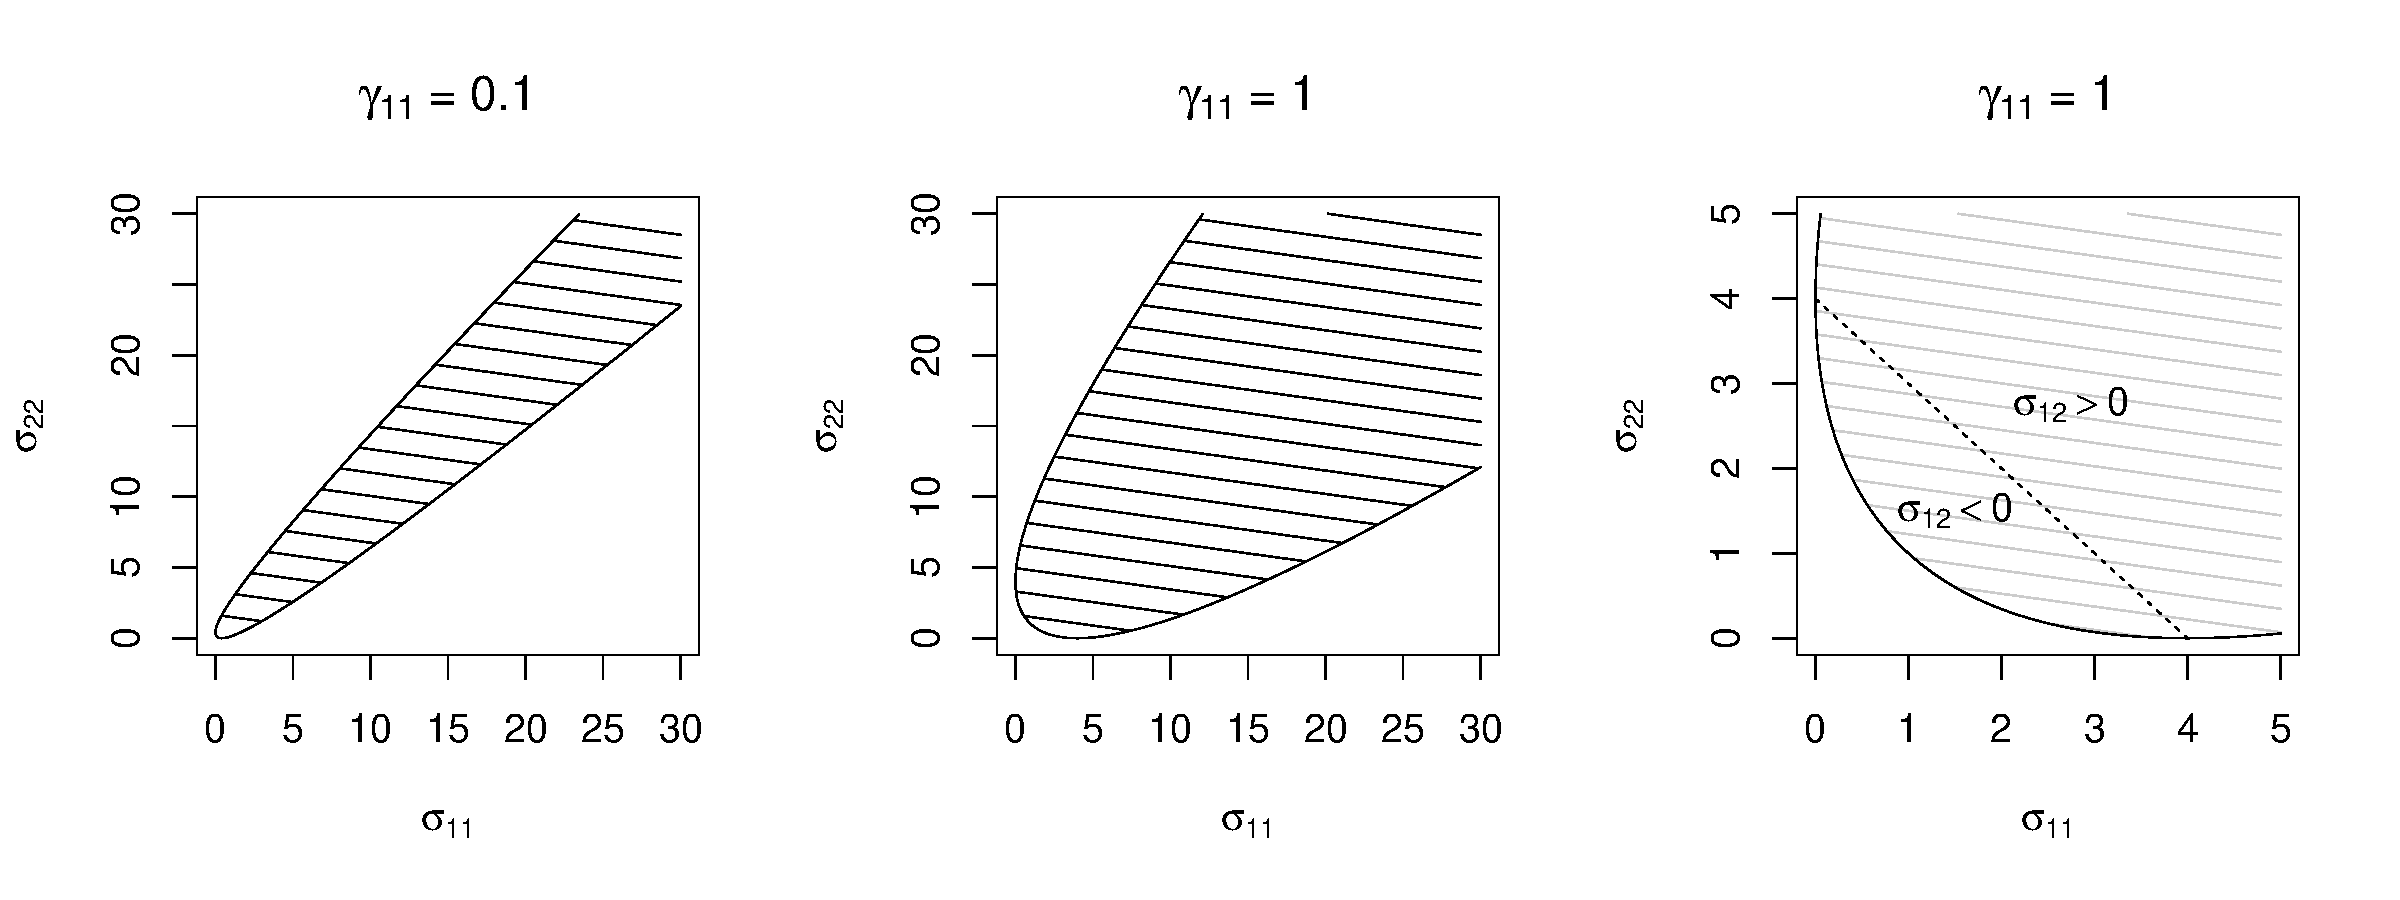
\includegraphics[width=6.5in]{figs/regions-2.pdf}
\begin{small}
\textit{Left and center: Region (shaded) where $\Sigma$ is positive definite, for $\gamma_{11} = 0.1$ and $\gamma_{11} = 1$. Right: Subregions where $\log X_1$ and $\log X_2$ are negatively correlated, uncorrelated, and positively correlated. Along the dashed line, $\sigma_{12} = 0$.}
\end{small}
\end{center}
\end{figure}

The region where $\Sigma$ is positive definite is plotted in Figure \ref{f:regions} for different values of $\gamma_{11}$. We can ask of this region of alternative covariance matrices, where in the region is the relationship between $\log X_1$ and $\log X_2$ positive or negative? Where are $\log X_1$ and $\log X_2$ independent? In the $p = 2$ case, the conditional and unconditional dependence relationships between $\log X_1$ and $\log X_2$ are the same, so we can simply examine $\sigma_{12}$. From equation (\ref{e:sig12}), we find that the boundary between the regions where $\sigma_{12} < 0$ and $\sigma_{12} > 0$ is the line
\begin{equation}
\sigma_{22} = 4\gamma_{11} - \sigma_{11}
\end{equation}

We can compare that line to the ``vertex" of the region, $(\gamma_{11}, \gamma_{11})$, which is found by solving for the point where the lower boundary intersects $\sigma_{22} = \sigma_{11}$. The vertex corresponds to $\Sigma = \Gamma$. As shown in Figure \ref{f:regions}, for any $\gamma_{11}$, there are always regions where $\sigma_{12} < 0$, $\sigma_{12} = 0$, and $\sigma_{12} > 0$.

Near or at the boundary of the region, the correlation is near or equal to $\pm 1$. Along the line $\sigma_{22} = \sigma_{11}$, the correlation goes from $-1$ at $(\gamma_{11}, \gamma_{11})$ to 0 at $(2\gamma_{11}, 2\gamma_{11})$ and approaches $+1$ as $\sigma_{11} = \sigma_{22}$ increases.

\subsubsection*{Generalizing to Larger $p$}

Characterizing the region where $\Sigma$ is positive definite is more difficult with $p > 2$, but the region can be explored for a particular $\Gamma$ by trial-and-error, choosing values for $\sigma_{11}, \dots, \sigma_{pp}$ and checking whether the minimum eigenvalue of $\Sigma$ is positive (indicating positive definiteness).

It appears that $\Sigma$ is positive definite for $(\sigma_{11}, \dots, \sigma_{pp}) = (\gamma_{11} + \delta, \dots, \gamma_{pp} + \delta)$ with any $\delta > 0$. For very small $\delta$, the entries of $\Sigma^{-1}$ are all or nearly all negative, corresponding to positive conditional relationships. As $\delta$ increases, the entries of $\Sigma^{-1}$ become all or nearly all positive, corresponding to negative conditional relationships. This pattern is similar to the pattern found in the $n = 2$ case.

It also appears to be true for larger $p$ that for fixed values of all $\sigma_{ii}$ except one, say $\sigma_{jj}$, $\Sigma$ is positive definite only for a fairly small interval of $\sigma_{jj}$ values.

What can be learned from these investigations is that for any given $\Gamma$ (or $\hat{\Gamma}$), there are potential log-absolute abundance covariance matrices which exhibit a wide variety of conditional and unconditional relationships among the variables and all could have resulted in $\Gamma$. What one would hope is that any valid $\Sigma$s which are quite different from $\Gamma$ represent implausible covariance structures, and that the $\Sigma$s which are plausible are also very similar to $\Gamma$ so that when graph selection is applied to $\Gamma$, its inferences are similar to what one would obtain if the absolute abundances were available. However, one may have little idea about which covariance structures are plausible or not.

\subsection*{Graph Selection Performance}

\begin{figure}
\caption{Band, cluster, and scale-free graph structures used in $p = 64$ simulations.}
\label{f:graphs}
\begin{center}
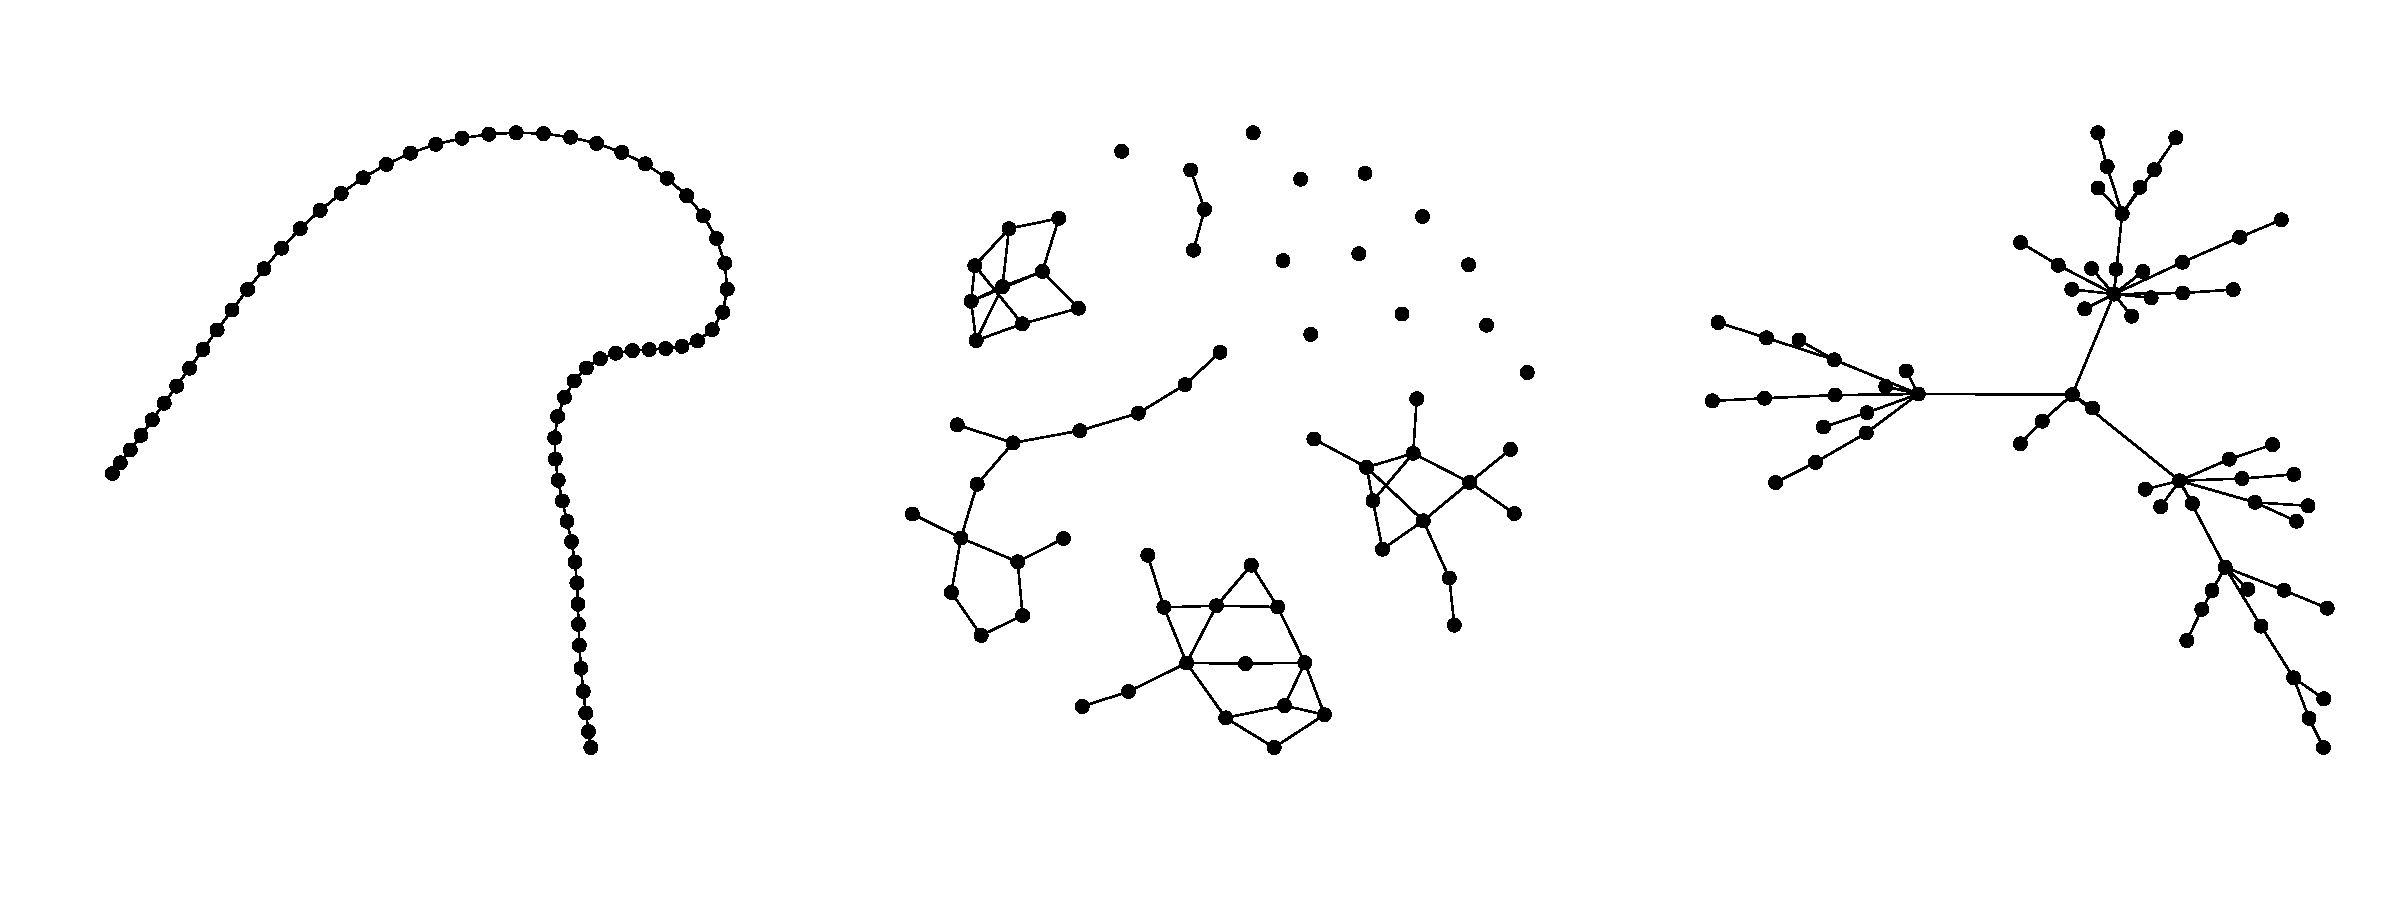
\includegraphics[width=6.5in]{figs/graphs-64.pdf}
\end{center}
\end{figure}

To assess the performance of graph selection under ideal conditions, I ran simulations using log-normal absolute abundances so that the log-absolute abundances had a multivariate normal distribution. For each of $p = 64$ and $p = 256$, samples were generated using a fixed precision matrix with the locations of non-zero entries determined by one of three graph structures: band, cluster, and scale-free. The graphs for $p = 64$ are shown in Figure \ref{f:graphs}. To control the strengths of the conditional relationships, all diagonal entries in the precision matrix were 4 and all off-diagonal entries were $\pm 1$. Thus, the partial correlations were all equal to $\pm 0.25$. The signs of the precision matrix entries were either all negative, half negative, or all positive. As noted above, a negative entry in the $(i,j)$ position of the precision matrix corresponds to a positive conditional dependence relationship between variables $i$ and $j$. That is, for fixed values of all other variables, variables $i$ and $j$ will have positive correlation when the entry in the precision matrix is negative and negative correlation when the entry is positive.

Performance was measured by the area under the precision-recall curve along the sequence of graphical lasso solutions for a decreasing sequence of $\lambda$ values. Precision and recall are calculated based on the numbers of true positives (TP), false positives (FP), and false negatives (FN) as expressed below.
\begin{equation}
\text{Recall} = \frac{\text{TP}}{\text{TP}+\text{FN}}\ \ \ \text{Precision} = \frac{\text{TP}}{\text{TP}+\text{FP}}
\end{equation}
Here, a true positive is when an edge exists in the true graph and is selected by graphical lasso. A false positive is when the edge does not exist but is selected, and a false negative is when the edge does exist but is not selected. For comparison, AUPR was also measured for graphical lasso performance using the log-abundance data before transformation.

This setup for the simulations was based on the simulations reported by Kurtz et al. \citeyear{kurtz}. The differences are that their simulations used count data mimicking microbial OTU counts from a real data set, they controlled the strength of OTU relationships using the condition number of the covariance matrix, and for every precision matrix entry in all trials, the sign was made positive with probability $\frac{1}{2}$ and negative otherwise. I observed that using their graph and precision matrix generator, for a fixed condition number, the partial correlations among variables tended to be much smaller for scale-free graphs compared to band and cluster graphs. I believe this explains the difference in performance among the graph types that they reported.

\begin{figure}
\caption{Graph selection performance with $p = 64$ and a scale-free graph structure.}
\label{f:perf64}
\begin{center}
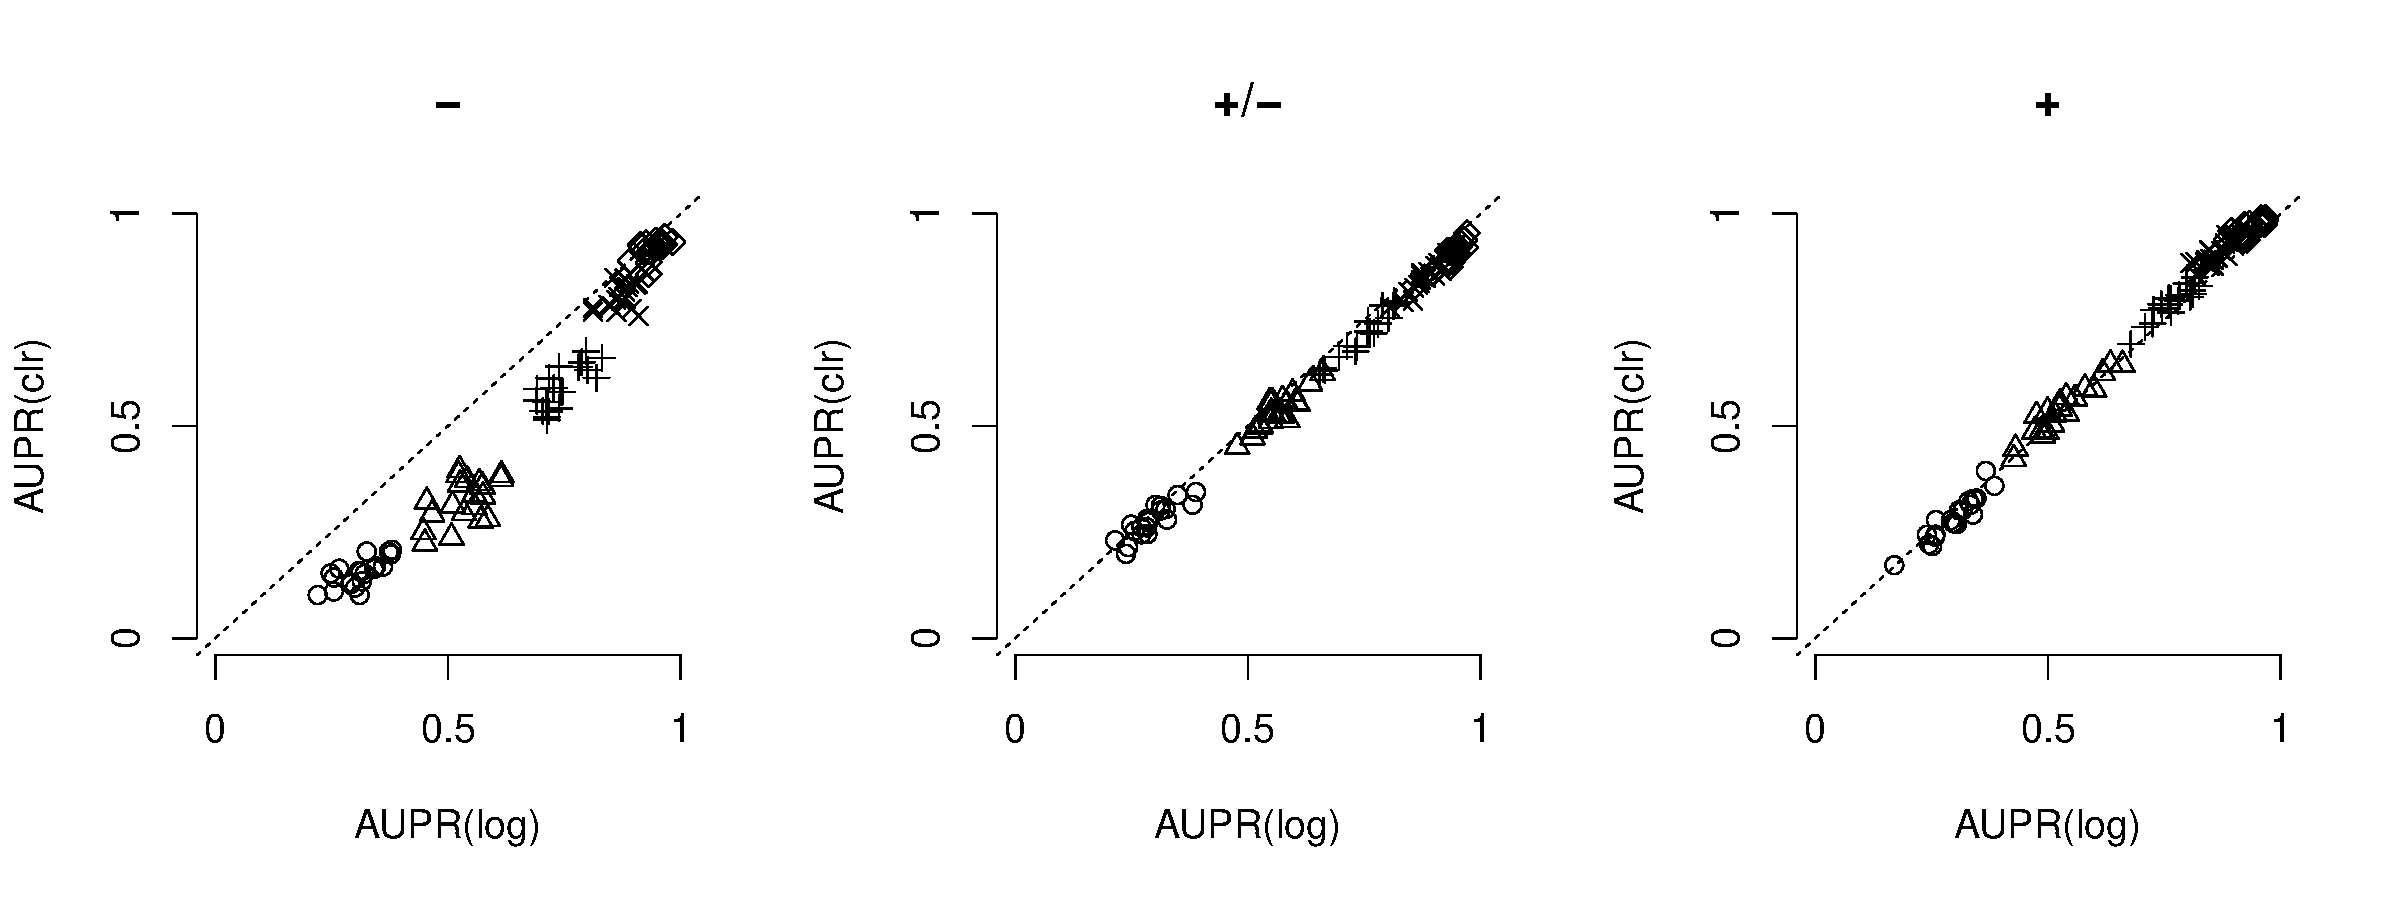
\includegraphics[width=6.5in]{figs/sim-64-scalefree.pdf}
\end{center}
\end{figure}

Besides sample size (performance steadily improved for both the log and clr data as $n$ increased from 32 to 512), the signs of the precision matrix entries had the largest effect on the performance of the graph selection. For $p = 64$, when all of the precision matrix entries were negative, graph selection using the clr abundance data underperformed compared to graph selection using the log abundances. The scale-free AUPR comparison is shown in Figure \ref{f:perf64}. However, for $p = 256$, performance is at least as good with clr data as with log data. Surprisingly, performance is sometimes slightly better with clr data for large $n$.

When all of the off-diagonal entries of the precision matrix are negative, all of the conditional relationships are positive, and the covariance matrix tends to have more and larger positive entries. As noted above, this results in a larger difference between $\Gamma$ and $\Omega$, which seems to result in worse graph selection performance, though the effect diminishes with larger $p$.

The conditions in these simulations were ideal in that $\Gamma$ does not differ from $\Omega$ in a way that affects graph selection too strongly. Essentially, the clr data are not too different from the log data. I performed additional simulations to investigate cases where the compositional effect is stronger. For the same graphs used in the $p = 64$ simulations above, I set the variance for $\log W_1$ to be 400 times as large as the other variances.

Under these conditions, where the variance of $\sum_{i=1}^p \log W_i$ is dominated by $\log W_1$, graph selection performs much worse on the clr data than on the log data. Graphical lasso selects many spurious edges between $\log W_1$ and the other $\log W_i$ because the clr transformation induces substantial changes in the covariances. Precision-recall curves for each graph structure and $n = 256$ are shown in Figure \ref{f:prcurves}. The edges selected in the case of the band graph using the log data are compared to the edges selected using the clr data in Figure \ref{f:spurious}.

\begin{figure}
\caption{Graph selection performance in the presence of one variance-dominating variable.}
\label{f:prcurves}
\begin{center}
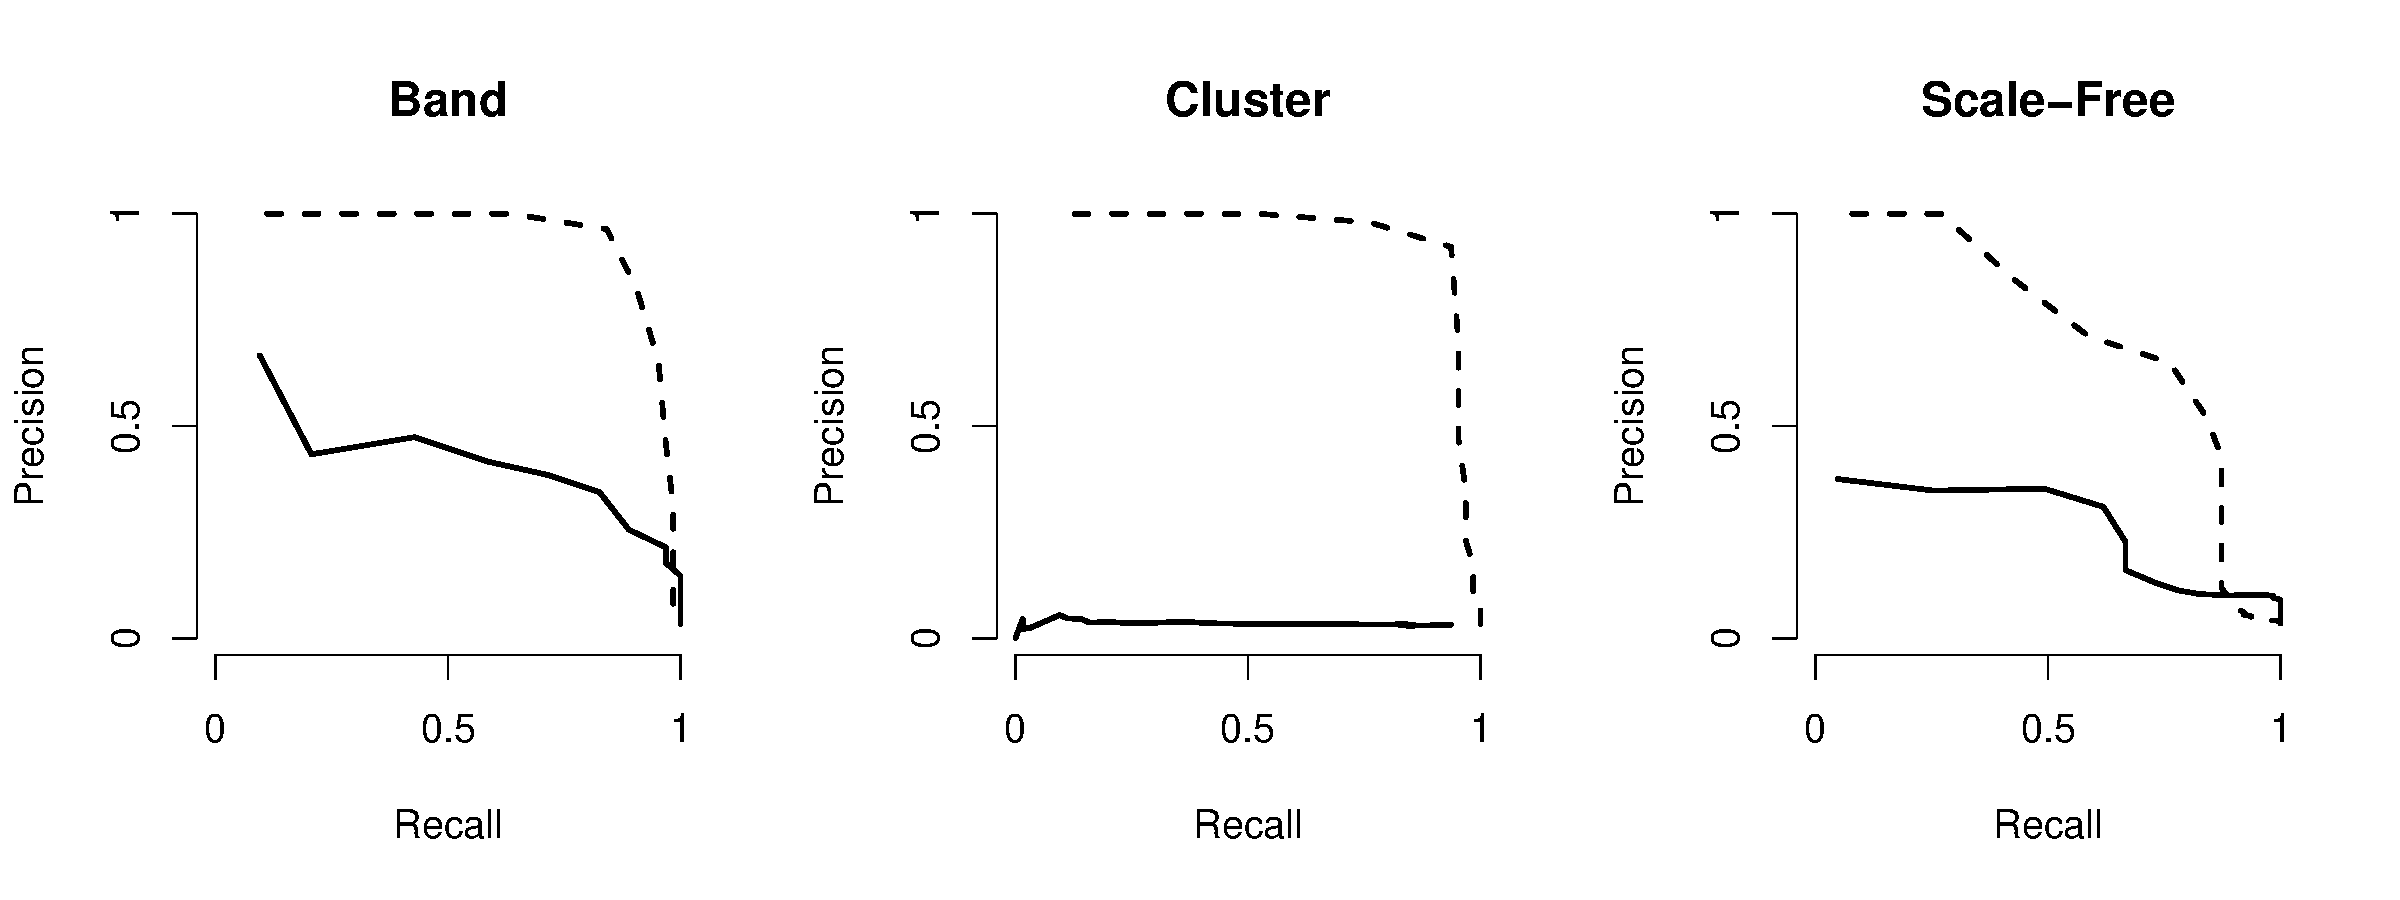
\includegraphics[width=6.5in]{figs/var-dom-pr.pdf}
\begin{small}
\textit{Precision vs. recall for graph selection from the clr abundance data} (-----) \textit{and log abundance data} (- - -).
\end{small}
\end{center}
\end{figure}

\begin{figure}
\caption{Spurious edges selected by graphical lasso.}
\label{f:spurious}
\begin{center}
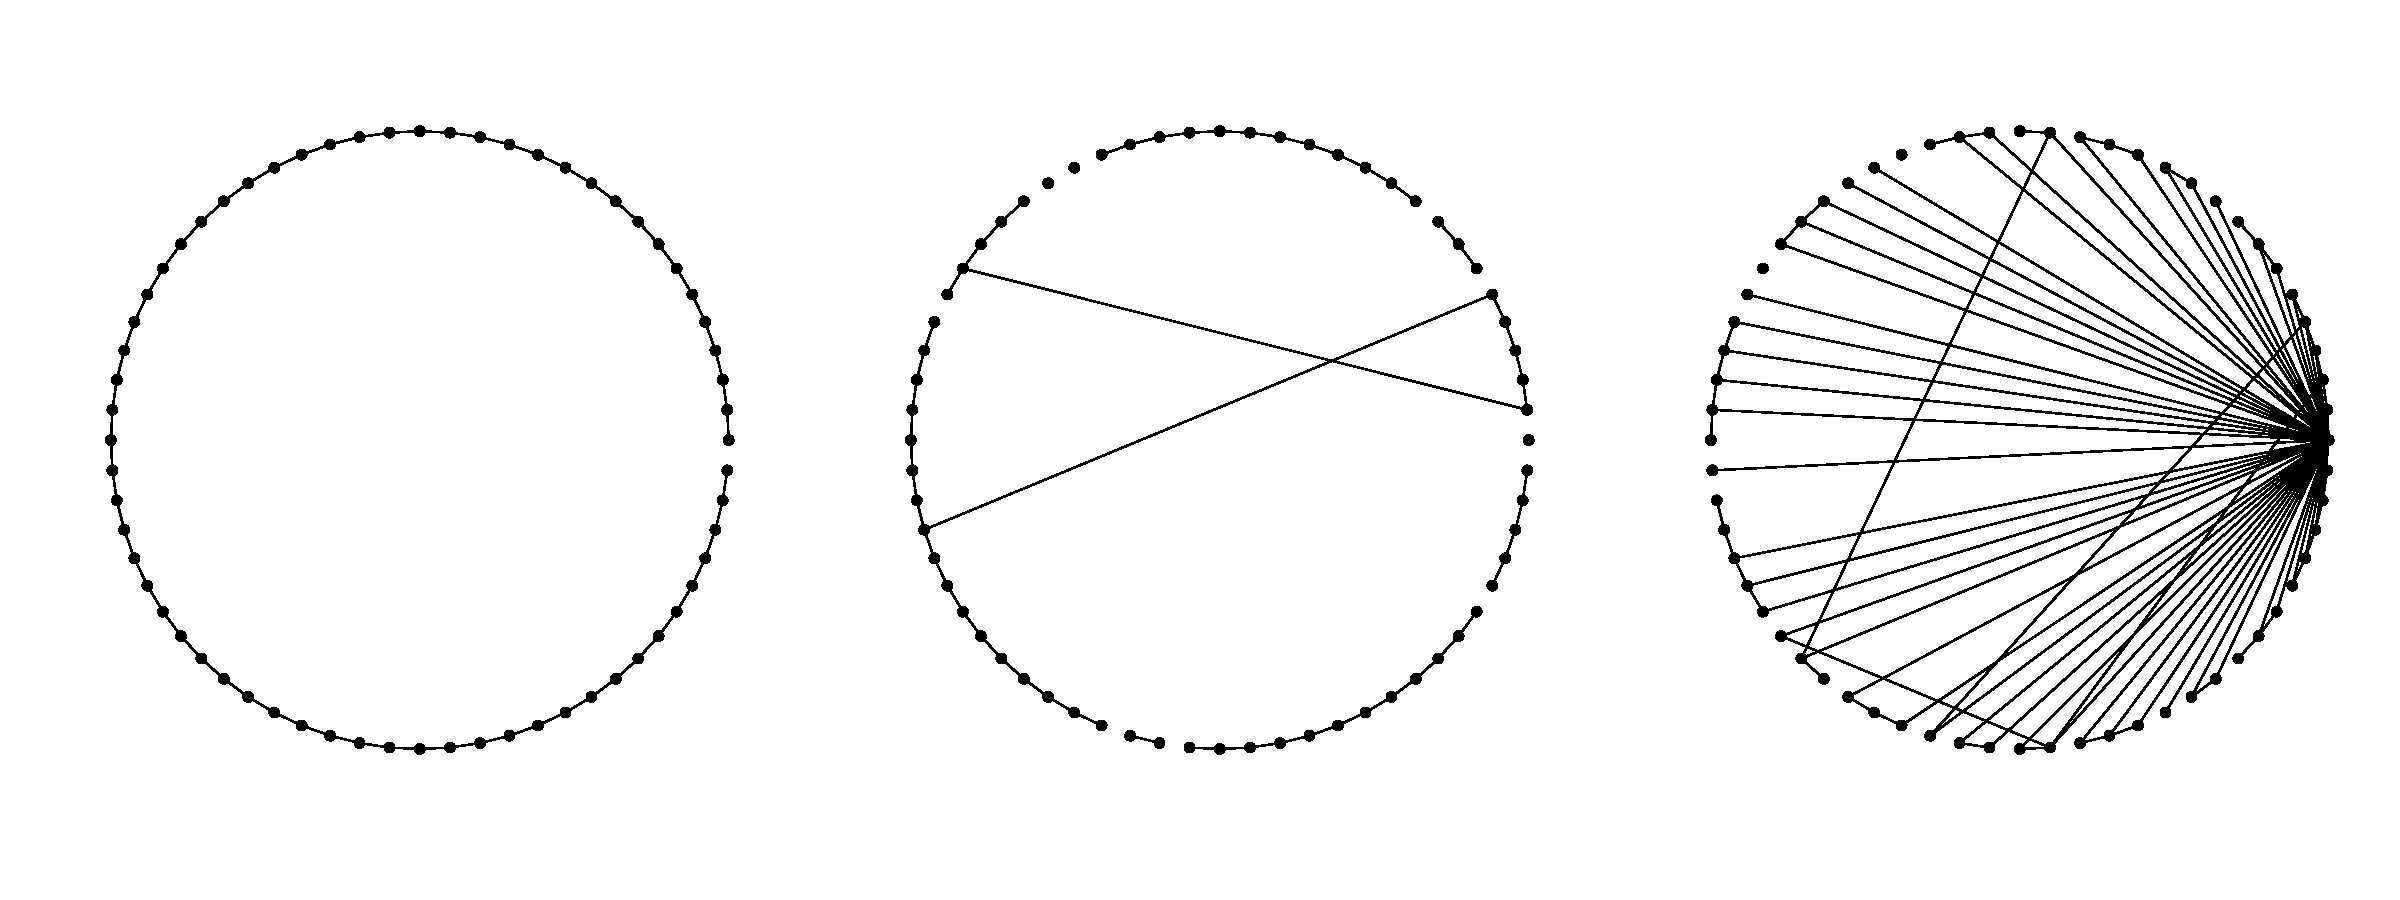
\includegraphics[width=6.5in]{figs/var-dom-band.pdf}
\begin{small}
\textit{Left: The true graph structure. Center: Edges selected by graphical lasso from the log abundance data, with lasso parameter $\lambda = 0.212$. Right: Edges selected from the clr abundance data with the same lasso parameter.}
\end{small}
\end{center}
\end{figure}

\subsection*{Discussion}

Compositional data derived from a basis of absolute abundances are fundamentally limited in the information they provide about the absolute abundances. Any analysis which is based on covariances in the compositional data, as is the case with the graph selection method considered here, must be used with the recognition that covariances in the compositional data may differ substantially from covariances in the basis abundances. I have shown that a variety of basis abundance structures exhibiting very different types of relationships among the variables can result in the same covariance structure in the clr-transformed compositional data.

Based on simulations, graph selection using clr-transformed compositional data works as well as (and occasionally even better than) the graph selection that would result from the log abundances for large $p$, provided that the compositional effect is not too strong. Strong compositional effects result when, for example, one variable or a group of variables dominates the variance of the sample totals. It is information about the sample totals which is lost when absolute abundances become compositional abundances. Therefore, any basis covariance patterns where the sample total is substantially dependent on the abundance patterns of a subset of variables can result in poor graph selection performance. If dependence relationships among variables are fairly sparse, and if the variances of the variables do not differ much, than moderate-to-large $p$ is sufficient for the compositional effects to be diminished or negligible.

\pagebreak
\bibliographystyle{biom}
\bibliography{paper}

\end{document}